\documentclass{article}
\usepackage{graphicx}
\title{Labwork 3}
\author{DAO HOANG DUNG \\ Student ID: 2540047}
\date{\today}

\begin{document}

\maketitle

\section{Objective}
For this labwork, I need to convert the RGB image to Grayscale image using both CPU and GPU.But instead of using 1D block,
I choose to improve by using 2D blocks.After that, I calculate the time to measure the speedup

\section{Python pseudo-code}
\begin{itemize}
     \item Read the image using plt.imread
     \item Reshape to 2D array
     \item Apply the grayscale for the image using CPU
     \item Apply the grayscale for the image using GPU
     \item Compare the different of time between each blocks
\end{itemize}


\section{Results}


\begin{figure}[htbp]
    \centering
    \begin{minipage}{0.48\textwidth}
        \centering
        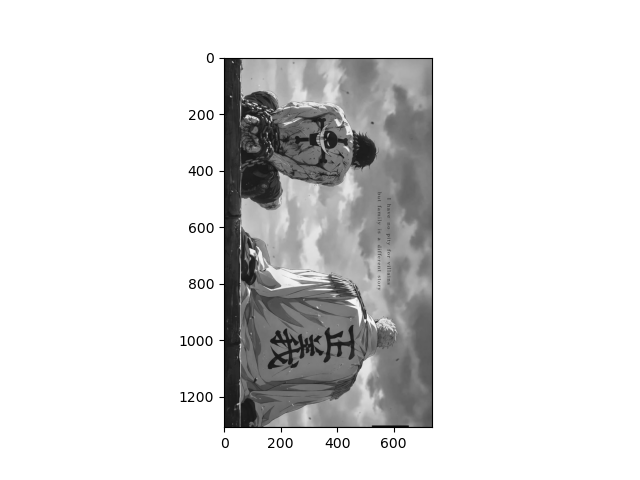
\includegraphics[width=\linewidth]{images/gray_cpu.png}
        \textbf{(a) CPU result}
    \end{minipage}
    \hfill
    \begin{minipage}{0.48\textwidth}
        \centering
        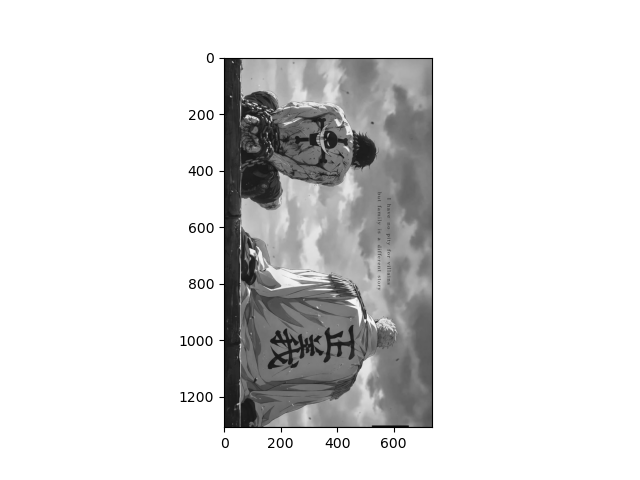
\includegraphics[width=\linewidth]{images/gray_gpu_128.png}
        \textbf{(b) GPU result}
    \end{minipage}
    \caption{Grayscale conversion results using the CPU and GPU.}
    \label{fig:grayscale-results}
\end{figure}



\begin{figure}[htbp]
    \centering
    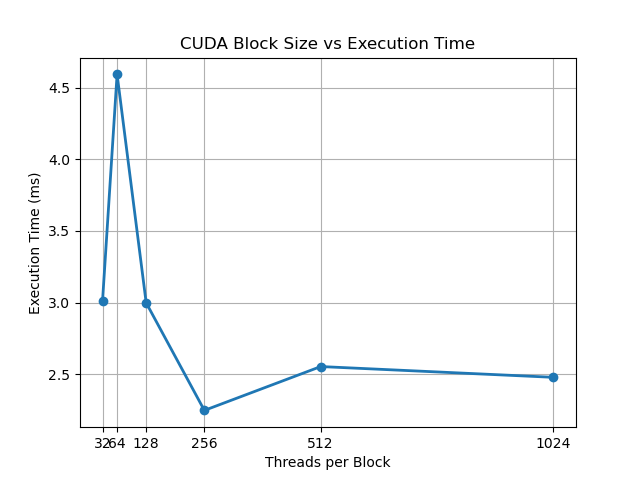
\includegraphics[width=0.8\textwidth]{images/plot.png}
    \caption{CUDA block size versus GPU execution time.}
    \label{fig:block-size-time}
\end{figure}

\end{document}
